\documentclass[conference]{IEEEtran}

\usepackage{cite}
\usepackage{amsmath,amssymb,amsfonts}
\usepackage{graphicx}
\usepackage{textcomp}
\usepackage{xcolor}
\usepackage{booktabs}
\usepackage{pifont}
\usepackage{tabularx}
\usepackage{enumitem}
\usepackage{tikz}
\usetikzlibrary{shapes.geometric, arrows, positioning, fit, backgrounds}
\usepackage{microtype}
\usepackage[hidelinks]{hyperref}

% Float and list spacing optimization for strict 2-page format
\setlength{\textfloatsep}{4pt plus 1.0pt minus 2.0pt}
\setlength{\floatsep}{4pt plus 1.0pt minus 2.0pt}
\setlength{\intextsep}{4pt plus 1.0pt minus 2.0pt}
\setlength{\dbltextfloatsep}{4pt plus 1.0pt minus 2.0pt}
\setlength{\abovecaptionskip}{2pt}
\setlength{\belowcaptionskip}{2pt}
\setlist{nosep,leftmargin=*}

% Tier status colors
\definecolor{tagimpl}{RGB}{20, 120, 20}
\definecolor{tagplan}{RGB}{185, 85, 0}
\definecolor{tagsel}{RGB}{15, 90, 180}

\begin{document}

\title{MANAR: A Pre-Flight Software Prototype, Route Optimization Heuristic, and Multi-Spectral Vision Benchmark for Aerial Search-and-Rescue\\
\Large\textit{Two-Page Technical Brief and Architecture Overview}}

\author{\IEEEauthorblockN{Oumar Ibrahim}
\IEEEauthorblockA{\textit{MANAR Search-and-Rescue Project} \\
United Arab Emirates}
}

\maketitle

\begin{abstract}
This brief presents MANAR (Multi-sensor Autonomous Navigation and Aerial Rescue), a pre-flight software prototype and supervised-autonomy framework for aerial Search-and-Rescue (SAR) robotics. Evaluated in-silico and on recorded video datasets prior to physical vehicle deployment, MANAR establishes a deterministic C++ control core, double-precision Haversine geodetics, an $O(n^2)$ greedy nearest-neighbor route optimizer with formal operator override privilege, sequential lawnmower sweeps, and an embedded ONNX Runtime visual detection pipeline. We present a 500-scenario route optimization evaluation against 2-opt, an empirical multi-spectral 26-video SAR benchmark ($>4\,200$ annotated frames) comparing YOLO11n against D-FINE-N, an analytical telemetry power model, and a systematic software verification matrix.
\end{abstract}

\begin{IEEEkeywords}
Search-and-Rescue UAVs, Supervised Autonomy, Deterministic Control, Greedy Route Optimization, Haversine Geodetics.
\end{IEEEkeywords}

\section{Introduction and System Maturity Tiers}
Search-and-Rescue (SAR) operations in remote wilderness and desert environments demand rapid aerial coverage under severe time constraints. Fully manual teleoperation overwhelms pilot cognitive capacity during multi-sensor tracking, while unconstrained autonomous systems introduce severe failure risks. MANAR resolves this trade-off through a \textbf{supervised-autonomy model} where deterministic flight logic and advisory perception operate under continuous human supervisory authority.

To establish rigorous engineering grounding, MANAR categorizes all capabilities across three distinct maturity tiers (Table~\ref{tab:maturity}):
\begin{enumerate}
    \item \textbf{Implemented Functional Prototype:} Fully compiled C++ logic, double-precision Haversine navigation, $O(n^2)$ greedy route optimization with operator override ($Y/N$), lawnmower sweeps, battery failsafes, and structured event logging.
    \item \textbf{Selected Closed Architecture:} Authoritative state ownership in C++, React/TypeScript interface via WebSocket + JSON, and on-demand Return-to-Launch (RTL) navigation semantics.
    \item \textbf{Planned Future Work:} PyTorch perception models, Mamba temporal fusion, PX4 SITL/HITL simulation, and field validation.
\end{enumerate}

\begin{table}[htbp]
\caption{MANAR Capability Maturity Status}
\label{tab:maturity}
\centering
\scriptsize
\begin{tabularx}{\columnwidth}{@{}lXl@{}}
\toprule
\textbf{Subsystem} & \textbf{Component / Function} & \textbf{Maturity Tier} \\
\midrule
\textbf{Control Core} & C++ Flight Logic (\texttt{control.exe}) & \textcolor{tagimpl}{\textbf{\ding{51} Implemented}} \\
\textbf{Navigation} & Double-Precision Haversine & \textcolor{tagimpl}{\textbf{\ding{51} Implemented}} \\
\textbf{Route Planner} & $O(n^2)$ Greedy NN + Override & \textcolor{tagimpl}{\textbf{\ding{51} Implemented}} \\
\textbf{Search Logic} & Lawnmower Grid Sequencing & \textcolor{tagimpl}{\textbf{\ding{51} Implemented}} \\
\textbf{Safety System} & Battery Failsafe Hierarchy & \textcolor{tagimpl}{\textbf{\ding{51} Implemented}} \\
\textbf{Visual CV} & YOLO11n + ORT C++ ($29.2\text{ ms}$) & \textcolor{tagimpl}{\textbf{\ding{51} Implemented}} \\
\textbf{CV Baseline} & D-FINE-N 26-Video Benchmark & \textcolor{tagimpl}{\textbf{\ding{51} Implemented}} \\
\midrule
\textbf{Operator GUI} & React / TypeScript Web UI & \textcolor{tagsel}{\textbf{\ding{115} Selected}} \\
\textbf{IPC Protocol} & WebSocket + JSON Transport & \textcolor{tagsel}{\textbf{\ding{115} Selected}} \\
\textbf{State Store} & Authoritative C++ Core Sync & \textcolor{tagsel}{\textbf{\ding{115} Selected}} \\
\midrule
\textbf{Candidate Track} & Kalman / ByteTrack MOT & \textcolor{tagplan}{\textbf{\ding{109} Planned}} \\
\textbf{Fusion Engine} & Mamba State Space Model & \textcolor{tagplan}{\textbf{\ding{109} Planned}} \\
\textbf{Autopilot} & PX4 SITL / HITL Simulation & \textcolor{tagplan}{\textbf{\ding{109} Planned}} \\
\textbf{Airframe} & Physical Flight Deployment & \textcolor{tagplan}{\textbf{\ding{109} Planned}} \\
\bottomrule
\end{tabularx}
\end{table}

\begin{figure}[t]
\centering
\resizebox{\columnwidth}{!}{%
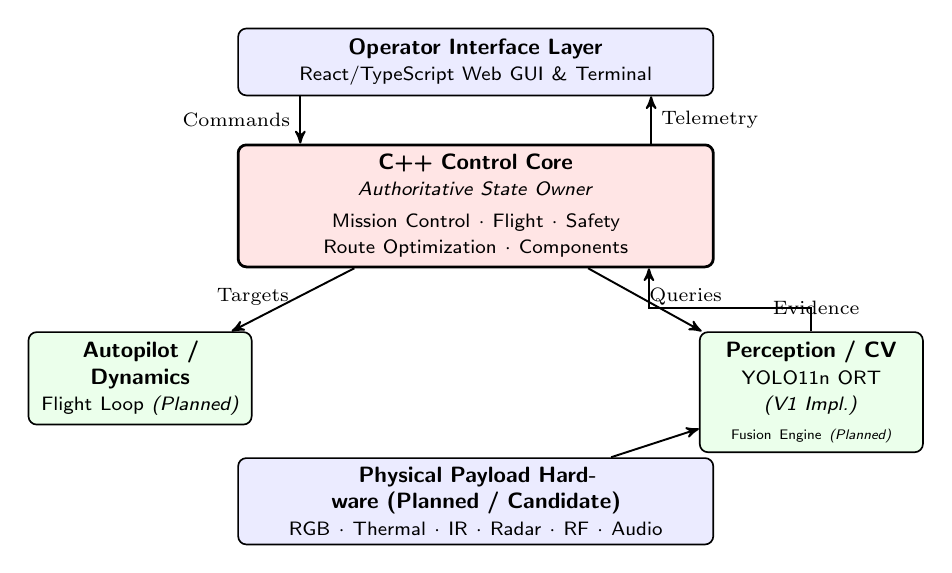
\begin{tikzpicture}[node distance=0.8cm, auto, >=stealth', font=\sffamily\footnotesize]
    \tikzstyle{block} = [draw, rectangle, fill=blue!8, text width=5.8cm, text centered, rounded corners=3pt, minimum height=0.85cm, line width=0.6pt]
    \tikzstyle{coreblock} = [draw, rectangle, fill=red!10, text width=5.8cm, text centered, rounded corners=3pt, minimum height=1.5cm, line width=1.0pt]
    \tikzstyle{subblock} = [draw, rectangle, fill=green!8, text width=2.6cm, text centered, rounded corners=3pt, minimum height=0.85cm, line width=0.6pt]

    \node [block] (gui) {\textbf{Operator Interface Layer}\\{\scriptsize React/TypeScript Web GUI \& Terminal}};
    \node [coreblock, below=0.6cm of gui] (core) {
        \textbf{C++ Control Core}\\
        {\scriptsize\textit{Authoritative State Owner}}\\[2pt]
        {\scriptsize Mission Control $\cdot$ Flight $\cdot$ Safety}\\
        {\scriptsize Route Optimization $\cdot$ Components}
    };
    \node [subblock, below left=0.8cm and -0.2cm of core] (autopilot) {\textbf{Autopilot / Dynamics}\\{\scriptsize Flight Loop \textit{(Planned)}}};
    \node [subblock, below right=0.8cm and -0.2cm of core] (perception) {
        \textbf{Perception / CV}\\
        {\scriptsize YOLO11n ORT \textit{(V1 Impl.)}}\\[1pt]
        {\tiny Fusion Engine \textit{(Planned)}}
    };
    \node [block, below=2.4cm of core] (sensors) {\textbf{Physical Payload Hardware \textit{(Planned / Candidate)}}\\{\scriptsize RGB $\cdot$ Thermal $\cdot$ IR $\cdot$ Radar $\cdot$ RF $\cdot$ Audio}};

    \draw [->, line width=0.7pt] (gui.south west) ++(0.8,0) -- ++(0,-0.6) node[left, font=\scriptsize, pos=0.5] {Commands};
    \draw [<-, line width=0.7pt] (gui.south east) ++(-0.8,0) -- ++(0,-0.6) node[right, font=\scriptsize, pos=0.5] {Telemetry};
    \draw [->, line width=0.7pt] (core) -- (autopilot) node[left, font=\scriptsize, pos=0.45] {Targets};
    \draw [->, line width=0.7pt] (core) -- (perception) node[right, font=\scriptsize, pos=0.45] {Queries};
    \draw [->, line width=0.7pt] (sensors) -- (perception) node[right, font=\scriptsize, pos=0.5] {};
    \draw [->, line width=0.7pt] (perception.north) ++(0,0) -- ++(0,0.3) -| ([xshift=2.2cm]core.south) node[right, font=\scriptsize, pos=0.15] {Evidence};
\end{tikzpicture}%
}
\caption{MANAR system architecture. The C++ Control Core is the authoritative state owner governing navigation, safety, and routing.}
\label{fig:system_architecture}
\end{figure}

\section{Implemented Deterministic C++ Core [Tier 1]}
The functional prototype (\texttt{core/}) executes deterministic navigation, route optimization, and safety monitoring:
\begin{enumerate}
    \item \textbf{Haversine Geodetics:} Exact surface distance calculation over spherical coordinates ($\phi, \lambda$):
    \begin{align}
    a &= \sin^2\left(\frac{\Delta\phi}{2}\right) + \cos\phi_1\cos\phi_2\sin^2\left(\frac{\Delta\lambda}{2}\right) \\
    d &= 2 R_E \operatorname{atan2}\left(\sqrt{a}, \sqrt{1-a}\right)
    \end{align}
    where $R_E = 6\,371\,000.0\text{ m}$.
    
    \item \textbf{Greedy Route Optimizer ($O(n^2)$):} For $n$ search locations, the planner iteratively selects the nearest unvisited target:
    \begin{align}
    p_{k+1} &= \arg\min_{p \in U_k} d(p_k, p) \\
    N_{\mathrm{eval}} &= \frac{n(n+1)}{2} = O(n^2)
    \end{align}
    For $n=8$, this evaluates 36 candidate distances ($8+7+\dots+1=36$) vs.\ $8! = 40\,320$ permutations. Operators retain an explicit override toggle ($Y/N$) to preserve manual tactical ordering.
    
    \item \textbf{Lawnmower Sector Sweeps:} Parameterized sweeps ($W \times H$, row spacing $\Delta y$) use exact local scaling constants:
    \begin{equation}
    M_{\mathrm{lat}} = 111\,320.0, \quad M_{\mathrm{lon}}(\phi_c) = 111\,320.0 \cos(\phi_c)
    \end{equation}
    
    \item \textbf{Battery Failsafe Hierarchy:} Continuous monitoring of simulated battery $B_k$: Warning ($30\%$), Recommend RTL ($25\%$), Emergency RTL ($15\%$), and Emergency Land ($5\%$).
\end{enumerate}

\begin{figure}[t]
\centering
\resizebox{\columnwidth}{!}{%
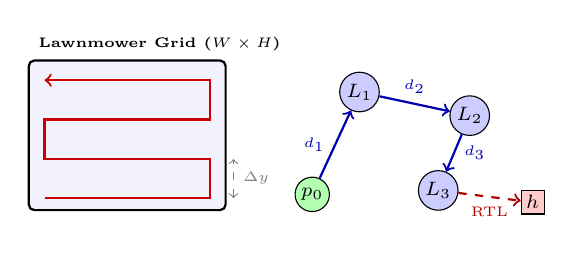
\begin{tikzpicture}[font=\sffamily\scriptsize]
    \draw[thick, fill=blue!5, rounded corners=2pt] (0,0) rectangle (2.5,1.9);
    \node[anchor=south west, font=\tiny\bfseries] at (0,1.9) {Lawnmower Grid ($W \times H$)};
    \draw[->, thick, red!80!black] (0.2,0.15) -- (2.3,0.15) -- (2.3,0.65) -- (0.2,0.65) -- (0.2,1.15) -- (2.3,1.15) -- (2.3,1.65) -- (0.2,1.65);
    \draw[<->, dashed, gray] (2.6,0.15) -- (2.6,0.65) node[midway, right, font=\tiny] {$\Delta y$};
    
    \begin{scope}[xshift=3.6cm, yshift=0.0cm]
        \node[draw, circle, fill=green!30, inner sep=1.2pt] (p0) at (0,0.2) {$p_0$};
        \node[draw, circle, fill=blue!20, inner sep=1.2pt] (L1) at (0.6,1.5) {$L_1$};
        \node[draw, circle, fill=blue!20, inner sep=1.2pt] (L2) at (2.0,1.2) {$L_2$};
        \node[draw, circle, fill=blue!20, inner sep=1.2pt] (L3) at (1.6,0.25) {$L_3$};
        \node[draw, rectangle, fill=red!20, inner sep=1.8pt] (home) at (2.8,0.1) {$h$};
        
        \draw[->, thick, blue!70!black] (p0) -- node[left, font=\tiny] {$d_1$} (L1);
        \draw[->, thick, blue!70!black] (L1) -- node[above, font=\tiny] {$d_2$} (L2);
        \draw[->, thick, blue!70!black] (L2) -- node[right, font=\tiny] {$d_3$} (L3);
        \draw[->, thick, dashed, red!70!black] (L3) -- node[below, font=\tiny] {RTL} (home);
    \end{scope}
\end{tikzpicture}%
}
\caption{Spatial geometry: Lawnmower sweep pattern (left) and sequential greedy route progression with Return-to-Launch final leg (right).}
\label{fig:lawnmower_and_route}
\end{figure}

\section{Multisensor Payload \& Perception [Tier 1 \& 3]}
MANAR incorporates eleven controllable payload categories for victim search, identification, and signaling (Fig.~\ref{fig:payload_capability_mapping}):

\begin{figure}[t]
\centering
\resizebox{\columnwidth}{!}{%
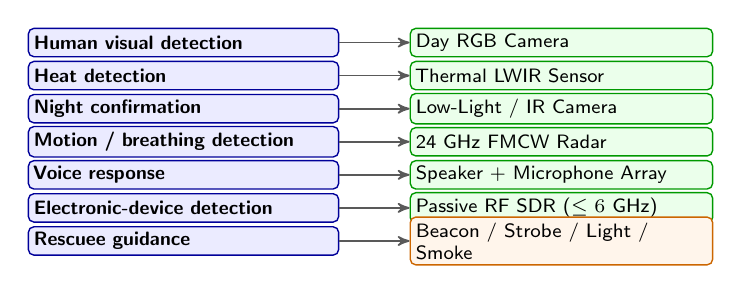
\begin{tikzpicture}[
    auto, >=stealth', font=\sffamily\scriptsize,
    role/.style={draw=blue!60!black, fill=blue!8, rounded corners=2pt, text width=3.8cm, minimum height=0.36cm, align=left, inner sep=2pt, line width=0.5pt},
    modality/.style={draw=green!60!black, fill=green!8, rounded corners=2pt, text width=3.7cm, minimum height=0.36cm, align=left, inner sep=2pt, line width=0.5pt},
    guide/.style={draw=orange!80!black, fill=orange!8, rounded corners=2pt, text width=3.7cm, minimum height=0.36cm, align=left, inner sep=2pt, line width=0.5pt},
    link/.style={->, line width=0.6pt, gray!70!black}
]
    \node[role] (r1) at (0, 2.52) {\textbf{Human visual detection}};
    \node[role] (r2) at (0, 2.10) {\textbf{Heat detection}};
    \node[role] (r3) at (0, 1.68) {\textbf{Night confirmation}};
    \node[role] (r4) at (0, 1.26) {\textbf{Motion / breathing detection}};
    \node[role] (r5) at (0, 0.84) {\textbf{Voice response}};
    \node[role] (r6) at (0, 0.42) {\textbf{Electronic-device detection}};
    \node[role] (r7) at (0, 0.00) {\textbf{Rescuee guidance}};

    \node[modality] (m1) at (4.8, 2.52) {Day RGB Camera};
    \node[modality] (m2) at (4.8, 2.10) {Thermal LWIR Sensor};
    \node[modality] (m3) at (4.8, 1.68) {Low-Light / IR Camera};
    \node[modality] (m4) at (4.8, 1.26) {24 GHz FMCW Radar};
    \node[modality] (m5) at (4.8, 0.84) {Speaker + Microphone Array};
    \node[modality] (m6) at (4.8, 0.42) {Passive RF SDR ($\le 6\text{ GHz}$)};
    \node[guide]    (m7) at (4.8, 0.00) {Beacon / Strobe / Light / Smoke};

    \draw[link] (r1.east) -- (m1.west);
    \draw[link] (r2.east) -- (m2.west);
    \draw[link] (r3.east) -- (m3.west);
    \draw[link] (r4.east) -- (m4.west);
    \draw[link] (r5.east) -- (m5.west);
    \draw[link] (r6.east) -- (m6.west);
    \draw[link] (r7.east) -- (m7.west);
\end{tikzpicture}%
}
\caption{Operational SAR capability to payload sensor and signaling subsystem mapping.}
\label{fig:payload_capability_mapping}
\end{figure}

\begin{itemize}
    \item \textbf{Visual Candidate Detection (YOLO11n):} Evaluated across 26 multi-spectral SAR video datasets ($>4\,200$ frames). Operates at $29.2 \pm 2.4\text{ ms}$ average latency ($34.2 \pm 2.8\text{ FPS}$ on CPU, $1.73\times$ faster than $50.5 \pm 4.1\text{ ms}$ D-FINE-N baseline) with $100\%$ clean negative rejection ($0\text{ FP}$) and superior concealed-target sensitivity ($44$ vs.\ $0$ detections).
    \item \textbf{Diurnal Optical Switching:} Sensor modes transition dynamically with hysteresis based on ambient light: $>150\text{ lx}$ (RGB+LWIR), $50\text{--}150\text{ lx}$ (RGB+IR+LWIR), and $<50\text{ lx}$ (IR+LWIR).
    \item \textbf{Acoustic Call-and-Listen Cycle [Tier 3]:} $35.4\text{ s}$ sequence ($8.4\text{ s}$ SOS buzzer, $12.0\text{ s}$ Arabic/English voice prompt, $15.0\text{ s}$ silent listening with motor-RPM harmonic cancellation).
    \item \textbf{Passive RF Two-Level Attention [Tier 3]:} Level 1 CFAR threshold ($N_{\mathrm{CFAR+}} \ge 3$) triggers Level 2 temporal trend tracking ($\Delta S_k$) in \texttt{Inspect} mode. Civilian operations subject to telecommunications statutory clearance.
    \item \textbf{FMCW Radar Theoretical Ranging [Tier 3]:} $24\text{ GHz}$ radar ($B \approx 250\text{ MHz}$) provides $\Delta R \approx c/(2B) \approx 0.60\text{ m}$ theoretical range resolution for breathing micro-motion.
    \item \textbf{Mamba SSM Alert Gate [Tier 3]:} Evaluates synchronized $10\text{ Hz}$ feature vectors $\mathbf{x}_t \in \mathbb{R}^D$ over $20\text{--}50$ frames ($2\text{--}5\text{ s}$). Mamba gates alert escalation; human operator assigns final rescue status.
    \item \textbf{Rescue Guidance [Tier 3]:} $360^\circ$ amber beacon, $2\text{ Hz}$ white strobe, spotlight, smoke marker, and 3 fixed heliograph mirrors ($40^\circ, 60^\circ, 75^\circ$).
\end{itemize}

\section{Adaptive Telemetry Power Model}
Analytical incremental RF transmission power $\Delta P_i$ across frequencies $f_i$ is formulated as:
\begin{equation}
\Delta P_i = (P_{\mathrm{TX}} - P_{\mathrm{RX}}) \cdot \left(\frac{8 \cdot B_i \cdot f_i}{R}\right) = \beta \cdot B_i \cdot f_i
\end{equation}
where $P_{\mathrm{TX}} = 4.8\text{ W}$, $P_{\mathrm{RX}} = 0.36\text{ W}$, $R = 64\text{ kbps}$, and slope factor $\beta \approx 5.55 \times 10^{-4}\text{ W}/(\text{byte}\cdot\text{Hz})$. Table~\ref{tab:telemetry_policy} summarizes the 14-stream dual-regime transmission policy.

\begin{table}[htbp]
\caption{Dual-Regime Telemetry Policy (14 Streams)}
\label{tab:telemetry_policy}
\centering
\scriptsize
\begin{tabular*}{\columnwidth}{@{\extracolsep{\fill}}lcrr@{}}
\toprule
\textbf{Stream Category} & \textbf{Payload ($B_i$)} & \textbf{Search} & \textbf{Proximity} \\
\midrule
Heartbeat / Position / Speed / Altitude & 24--28 B & 2.0 Hz & 5.0 Hz \\
Heading & 22 B & 1.0 Hz & 5.0 Hz \\
Battery Percentage & 22 B & 0.2 Hz & 0.5 Hz \\
Flight / Mission / Component State & 21--24 B & On Change & On Change \\
Raw Sensor Measurements & 52 B & Local & 5--10 Hz \\
Confidence Alerts / Failsafes & 28--32 B & Event & Event \\
Diagnostics / Logs / Config & 84 B & Pull & Pull \\
\bottomrule
\end{tabular*}
\end{table}

\section{Verification and System Roadmap}
\textbf{Software Prototype Verification:} Software-in-the-loop integration testing confirmed deterministic C++ control flow, search plan locking, start rejection on empty plans, Return-to-Launch (RTL) preemption, and real-time ONNX Runtime visual candidate detection under Windows 11 / GCC.

\textbf{System Roadmap:}
\begin{enumerate}
    \item \emph{Interface Layer:} Complete React/TypeScript WebSocket GCS.
    \item \emph{Perception Tracking \& Fusion:} Implement Kalman / ByteTrack tracking and Mamba temporal fusion.
    \item \emph{Autopilot Integration:} PX4 SITL simulation followed by HITL physical airframe flight testing.
\end{enumerate}

\end{document}
